\scanpage{95}
% archive foliation: 97
structures réelles s'identifie à $G^-$, qui est un \uline{torseur}
sous $G^+$ par translations à gauche. Par contre,
l'opération de $G^+$ sur $G^-$ par autos intérieurs est
\unsure{pas} libre, le centre $\zeta\simeq\{\pm1\}$ de $G$ opère trivialement,
et il y a deux orbites sous $G^+$ (ou encore $G^+/\zeta$).
Ce sont (pour $n=4$ ou $6$) les symétries par rapport
\deleted{\unsure{Dans un}\unsure{ premier}} respectivement aux sommets et aux centres
des \deleted{\unsure{ce}} polygone (carré ou hexagone) fondamental.
\figure{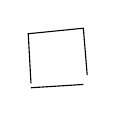
\begin{tikzpicture}[scale=.7]\draw (0,0)--(-.05,.9)--(.95,1)--(1.02,.15);\draw (0,-.08)--(.95,-.02);\end{tikzpicture}}

\uuline{Donc} en résumé

\uline{Proposition} Soit une courbe elliptique \deleted{réelle} complexe. \inserted{$X$}
\deleted{Pour qu'elle admette des}\inserted{Les} structures réelles \deleted{\unsure{sur}\unsure{ elle}}.
\deleted{qu'elles} correspondent aux \inserted{anti} autos \deleted{involutifs} de la
courbe \inserted{elliptique} conforme \deleted{\unsure{fournis}\unsure{ qu'il y en a}},\inserted{il y en a} si et seulement
si la suite
\diagram{\begin{tikzcd}[ampersand replacement=\&]
\unsure{0|1}\arrow[r,dash]\&G^+\arrow[r,dash]\&G\arrow[r,dash]\&\pm1\arrow[r,dash]\&\unsure{0|1}
\end{tikzcd}}
est exacte (à droite). Dans ce cas, $G$ est \deleted{\unsure{un}}\inserted{isom. au} groupe diédral
\inserted{$D_n$} dont $G^+$ (d'ordre $n=2,4$ ou $6$) est le groupe des rotations.
L'ens des structures réelles se partage en deux
orbites sous $G^+$ (opérant par autos intérieurs), et
les structures réelles correspondant à deux orbites
distinctes sont (par définition !) non isomorphes. \deleted{\unsure{et les}
deux orbites correspondent aux structures $E_a,E'_a$}

Je présume que si l'une est formée de structures
$E_a$ ($a\in\mathbb R^{*+}$ fixé), l'autre est formée des structures $E'_{\unsure{a|b}}$
(avec $b\unsure{=|\ne}a$), et inversement, i.e. qu'on peut trouver
un $a\in\mathbb R^{*+}$ unique, tel que les deux orbites sont
l'une formée de structures isom. à $E_a$, l'autre de
structures isom. à $E'_a$. De plus il faudrait
